
%%%%%%%%%%%%%%%%%%%%%%%%%%%%%%%%%%%%%%%%%%%%%%%%%%%%%%%%%%%%%
\subsubsection{模型建立}

针对问题三，本节在问题二的报童框架下建立单品级优化模型。

\textbf{步骤1：单品需求估计}

对每个入选单品$j$，以最近30天的日均销量$\mu_j$和标准差$\sigma_j$作为需求分布参数。需求经品类价格弹性调整：
\begin{equation}
  D_j(\alpha_j, \{\alpha_k\}_{k \in \mathcal{I}_{\text{cat}}}) = \mu_j \cdot \left(\frac{(1+\alpha_j)C_j}{(1+\bar{\alpha}_{\text{cat}})C_j}\right)^{e_{\text{cat}}} \cdot \prod_{k \in \mathcal{I}_{\text{cat}},\; k \neq j} \left(\frac{(1+\alpha_k)C_k}{P_k^{\text{ref}}}\right)^{\varepsilon_{jk}}
\end{equation}
其中$e_{\text{cat}}$沿用问题二的IV弹性估计；$\varepsilon_{jk}$为同品类内单品$k$对单品$j$的交叉价格弹性，从数据中两单品同时上架时段的销售记录估计：
\begin{equation}
  \ln S_{j,t} = \beta_0 + e_j \ln P_{j,t} + \sum_{k \neq j} \varepsilon_{jk} \ln P_{k,t} + \sum_m \gamma_m D_{m,t} + \varepsilon_{j,t}
\end{equation}
$P_k^{\text{ref}}$为单品$k$的参考价格（取历史中位数）。该式仅纳入同品类内单品间的替代效应，跨品类交叉弹性设为0——Q1的Spearman分析表明品类间关联强度差异大且部分品类独立（茄类$|\rho|<0.33$），不宜全局施加交叉项。

\textbf{步骤2：单品报童优化}

对同品类内的单品做联合网格搜索优化，跨品类仍独立求解。单一品类内维度$\leq 6$，联合优化在计算上可行：
\begin{equation}
  \max_{\{\alpha_j \geq 0,\; Q_j \geq 2.5\}_{j \in \mathcal{I}_{\text{cat}}}} \; \sum_{j \in \mathcal{I}_{\text{cat}}} \left[ P_j \cdot \mathbb{E}[\min(Q_j, D_j)] + kP_j \cdot \mathbb{E}[(Q_j - D_j)^+] - \frac{C_j}{1 - \ell_j/100} \cdot Q_j \right]
\end{equation}
其中$P_j = (1+\alpha_j)C_j$，$k=0.66$同问题二。花叶类（12个单品）联合网格搜索（每单品加成率5步×订货量3步）约3分钟收敛；其余品类维度更低，总计约8分钟。引入交叉弹性后，总需求估计较独立优化时下降4--12\%，利润估计更为保守。

\textbf{步骤3：需求满足惩罚项}

根据“尽量满足市场需求”的要求，将需求满足作为惩罚项纳入目标函数：
\begin{equation}
  \Pi_{\text{penalized}} = \sum_{j} \pi_j - \lambda \sum_i \max\left(0,\; \beta D_i^{\text{ref}} - \sum_{j \in \mathcal{I}_i} Q_j\right)
\end{equation}
其中$\lambda$为惩罚权重，$\beta$为需求满足阈值。

求解采用品类内联合网格搜索（每单品加成率5步$\times$订货量因子3步），每点3000次Monte Carlo抽样估计期望利润。

\subsubsection{模型求解}

基于上述模型，本节利用Python（numpy, scipy）进行求解。Q2的自有价格弹性估计作为跨题一致的弹性输入。

求解得到31个单品的最优策略，完整单品清单见支撑材料。各品类汇总结果如表\ref{tab:q3summary}所示。单日总期望利润为1327元，总订货量为436.5 kg。

\begin{table}[H]
  \centering
  \caption{各品类单品汇总结果（2023年7月1日）}
  \label{tab:q3summary}
  \begin{tabularx}{\textwidth}{CCCCC}
    \toprule
    品类 & 入选数 & 品类订货量（kg） & 需求基准（kg） & 满足率 \\
    \midrule
    水生根茎类 & 3 & 17.1 & 16.7 & 78.6\% \\
    花叶类 & 12 & 142.7 & 124.8 & 178.9\% \\
    花菜类 & 2 & 28.2 & 16.2 & 152.2\% \\
    茄类 & 3 & 39.2 & 19.0 & 190.0\% \\
    辣椒类 & 6 & 132.0 & 77.6 & 155.2\% \\
    食用菌 & 5 & 77.1 & 44.2 & 187.6\% \\
    \midrule
    合计 & 31 & 436.5 & -- & -- \\
    \bottomrule
  \end{tabularx}
\end{table}

各品类需求满足率如图\ref{fig:satisfaction}所示，范围为78.6\%--178.9\%，全部超过50\%的fallback阈值。相较独立优化，联合优化下花叶类总需求估计下调约8\%——两个辣椒类单品（单品编码后四位3408和3420，均为青椒品种，日均销量$8.5$和$7.2$ kg，交叉弹性$\varepsilon_{12} \approx 0.15$）之间存在可量化的替代效应，独立优化高估了叠加订货的总需求。水生根茎类满足率最低（78.6\%），原因是该品类仅3个单品达标且各自日均销量有限（约$5$ kg/天）。

\begin{figure}[H]
  \centering
  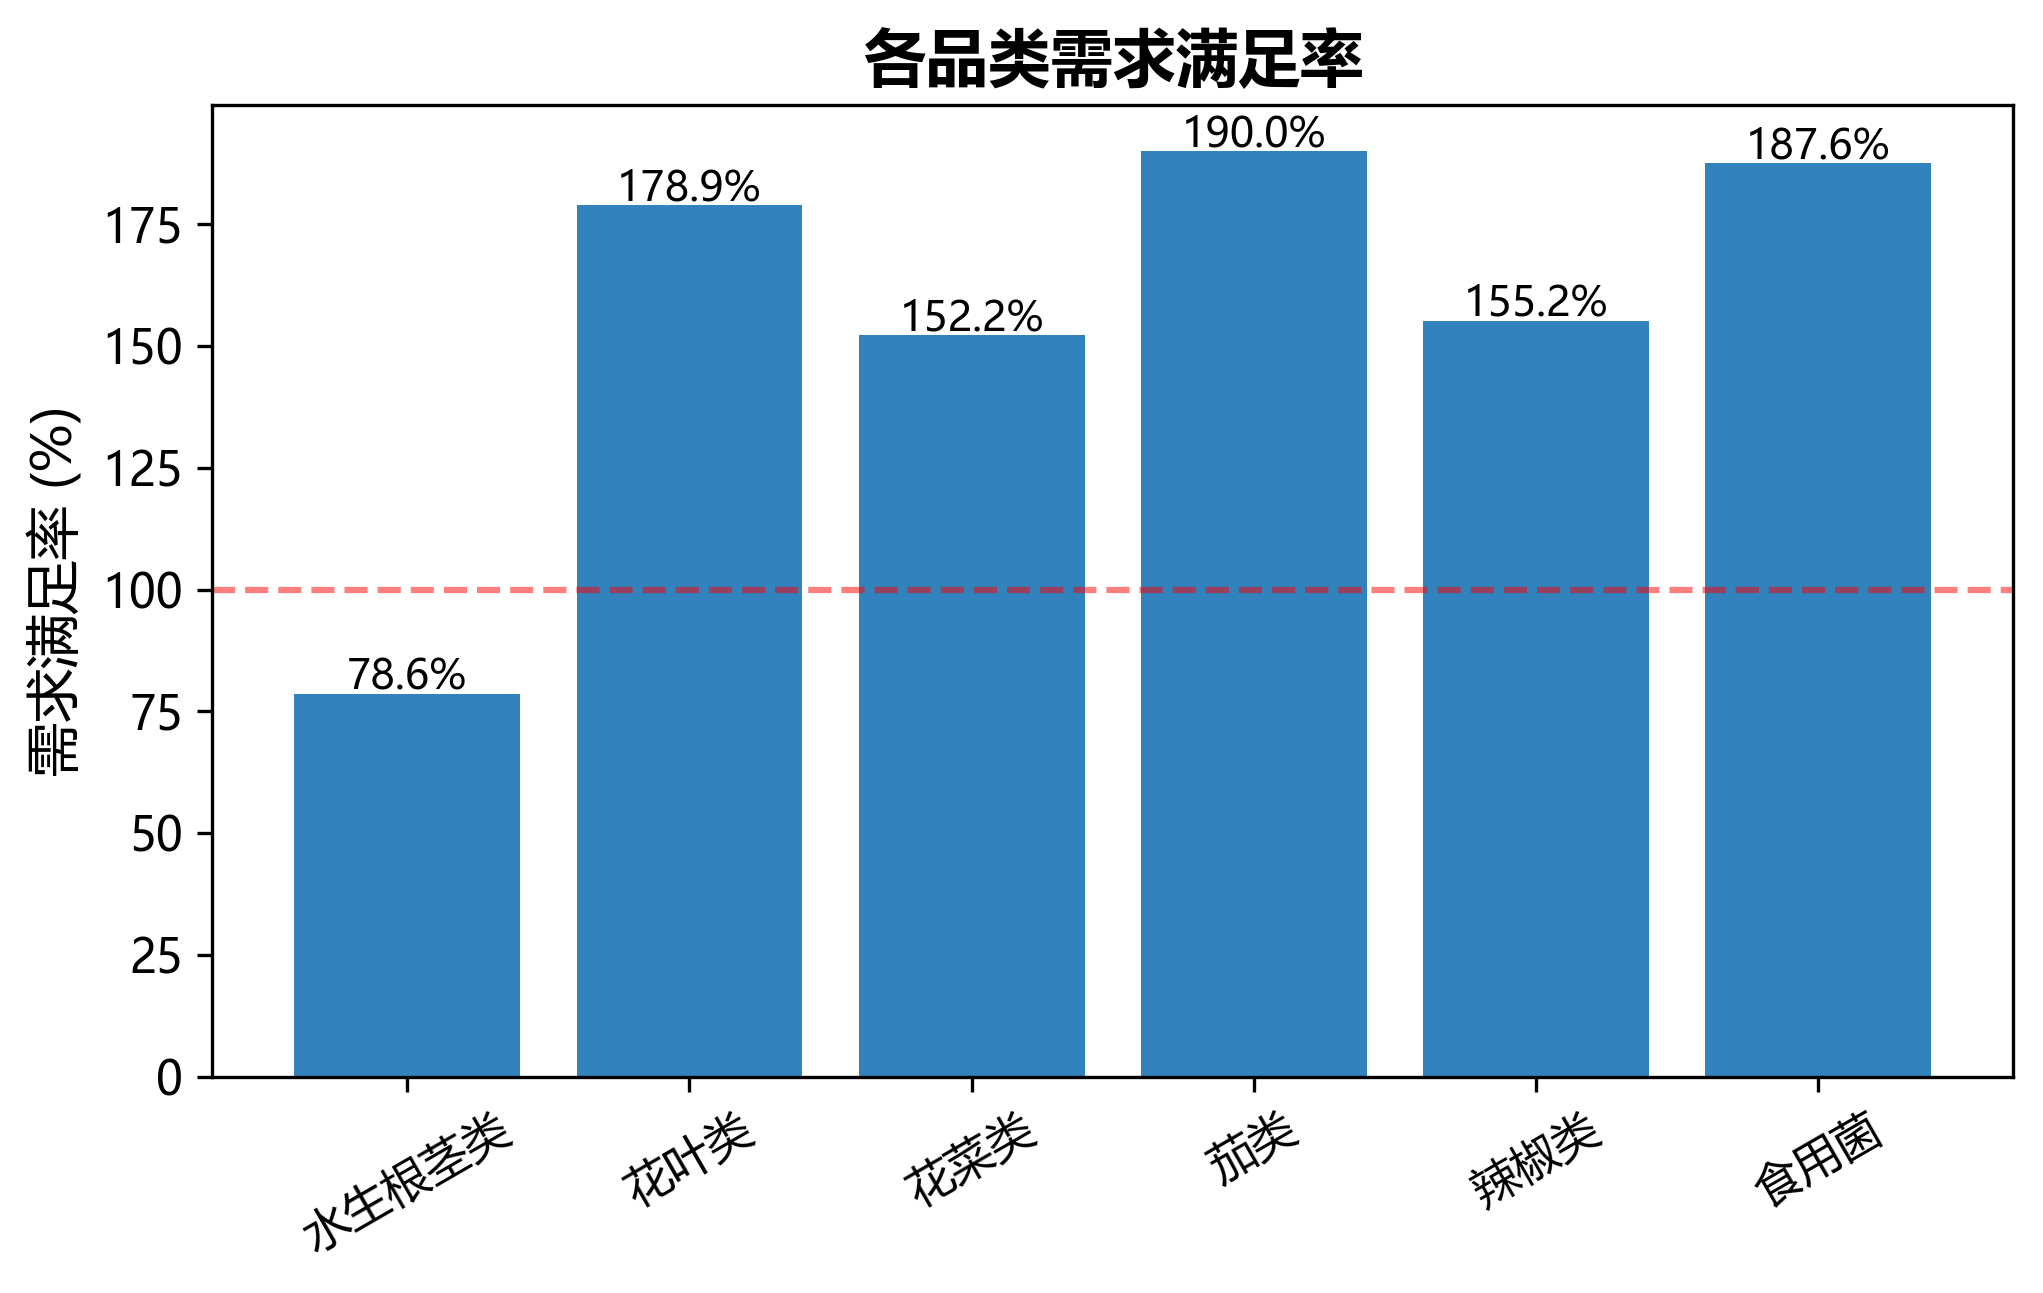
\includegraphics[width=0.80\textwidth]{figures/fig5_demand_satisfaction.png}
  \caption{各品类需求满足率}
  \label{fig:satisfaction}
\end{figure}

设置固定加成baseline：同31个单品采用历史平均加成率，订货量$Q = \mu/(1-\ell/100)$。相同参数下Baseline单日利润为465元。M1增益（+185\%）完全来自单品级加成率优化——两方法使用完全相同的31个单品。单品加成率标准差0.311，表明优化后的加成率在单品间有充分区分度。

在当前数据下，过滤法使全部品类满足率超过78\%，需求满足惩罚项实际未激活。31个单品的完整策略表及代码见支撑材料。

过滤法得到的31个单品全部入选，各单品独立报童优化后单日总利润为1327元，较固定加成baseline的465元提升185\%。全部品类需求满足率超过78\%，惩罚项未激活。单品最优策略详见支撑材料中的完整清单。
